\documentclass[12pt]{scrartcl}
\usepackage[ngerman, english]{babel}
\usepackage[T1]{fontenc}
\usepackage[utf8]{inputenc}
\usepackage[color=yellow!15]{todonotes}
\usepackage{graphicx}

% The following parameters seem to provide a reasonable page setup.
\topmargin 0.0cm
\oddsidemargin 0.2cm
\textwidth 16cm 
\textheight 21cm
\footskip 1.0cm


%The next command sets up an environment for the abstract to your paper.
\newenvironment{sciabstract}{%
\begin{quote} \bf}
{\end{quote}}


% If your reference list includes text notes as well as references,
% include the following line; otherwise, comment it out.

\renewcommand\refname{References and Notes}

% The following lines set up an environment for the last note in the
% reference list, which commonly includes acknowledgments of funding,
% help, etc.  It's intended for users of BibTeX or the {thebibliography}
% environment.  Users who are hand-coding their references at the end
% using a list environment such as {enumerate} can simply add another
% item at the end, and it will be numbered automatically.

\newcounter{lastnote}
\newenvironment{scilastnote}{%
\setcounter{lastnote}{\value{enumiv}}%
\addtocounter{lastnote}{+1}%
\begin{list}%
{\arabic{lastnote}.}
{\setlength{\leftmargin}{.22in}}
{\setlength{\labelsep}{.5em}}}
{\end{list}}


% Include your paper's title here

\title{\textbf{ \Large{Decentralized, autonomous sensor fault detection using neural networks}} }


\author
{Katrin Jahr, Robert Schlich$^{1}$\\
\\
\normalsize{$^{1}$Degree program “Civil Engineering” (M.Sc.)}\\
\normalsize{Bauhaus-Universität Weimar, Germany}\\
\\
\normalsize{katrin.jahr@uni-weimar.de}\\
\normalsize{robert.schlich@uni-weimar.de}
}


% Include the date command, but leave its argument blank.
\date{}



%%%%%%%%%%%%%%%%% END OF PREAMBLE %%%%%%%%%%%%%%%%



\begin{document} 

% Double-space the manuscript.

\baselineskip24pt

% Make the title.

\maketitle 



% Place your abstract within the special {sciabstract} environment.

\begin{sciabstract}


The dependability and the accuracy of structural health monitoring systems are significantly affected by sensor faults. 
In this paper, the design and implementation of a wireless structural health monitoring system, capable of decentralized autonomous fault detection, is presented. 
For self-detecting sensor faults, each sensor node predicts its expected sensor data and compares it to measured sensor data. 
The predictions are computed using neural networks with measured data of adjacent sensor nodes.
In laboratory experiments, devised to validate the proposed approach, several simulated sensor faults are detected.
These results indicate that the use of neural networks increases the dependability and the accuracy of structural health monitoring systems.


%1st Draft:
%The dependability and the accuracy of structural health monitoring systems are significantly affected by sensor faults. Autonomous fault detection can be obtained by comparing sensor data with data predicted by neural networks. In this paper, the design and implementation of a wireless structural health monitoring system capable of autonomous sensor fault detection using a neural network is presented. The system was validated in laboratory experiments showing its efficency.

%2nd Draft
%The dependability and the accuracy of structural health monitoring systems are significantly affected by sensor faults. In this paper, the design and implementation of a wireless structural health monitoring system is presented. A neural network is used for autonomous fault detection by comparing the predicted data with measured sensor data. In laboratory experiments, sensor faults were detected reliably, proving that the use of neural networks increases the reliability of structural health monitoring systems.

%3th Draft 
%The dependability and the accuracy of structural health monitoring systems are significantly affected by sensor faults. In this paper, the design and implementation of a wireless structural health monitoring system, capable of autonomous fault detection, is presented. A neural network is used for self-monitoring of each sensor by predicting data values and comparing these values to measured sensor data. In laboratory experiments, sensor faults were detected reliably, proving that the use of neural networks increases the reliability of structural health monitoring systems.

%4th Draft
%The dependability and the accuracy of structural health monitoring systems are significantly affected by sensor faults. 
%In this paper, the design and implementation of a wireless structural health monitoring system, capable of autonomous fault detection, is presented. 
%A neural network is used for self-monitoring of each sensor node by predicting the measured data with data values submitted by adjacent sensor nodes. 
%These predictions are then compared to the measured data.
%In laboratory experiments, sensor faults were detected, proving that the use of neural networks increases the reliability of structural health monitoring systems.



\end{sciabstract}

\section*{Dictionary}

\begin{tabular}{|l|l|}
\hline 
Sensorknoten (SunSPOT) & sensor node \\ 
\hline 
einzelner Messsensor (Thermometer) & sensor \\ 
\hline 
Knoten im neuronalen Netz & neuron \\ 
\hline 
eine abgeschlossene Messung & measurement \\ 
\hline 
gemessene Werte & sensor data \\ 
\hline 
vorhergesagte Werte & predicted data \\ 
\hline 
durch Vorhersage erwartete Werte & expected data \\ 
\hline 
einzelner Messwert & measurement value \\ 
\hline 
\end{tabular} 

%----------------------------------------------------------------------------------------

\section*{Introduction}

\begin{itemize}
\item Unfälle gefährden Menschenleben und sind teuer
\item SHMS können Unfälle verhindern
\item kabellose Sensoren sind besser
\item Sensoren sind fehleranfällig
\item Lösung: autonome Fehlererkennung 
\item Lösungsansätze mit Literaturbelegen
\item Ansatz: Neuronales Netz
\item Überblick, Vorteile
\item Literatur zu neuronalen Netzen
\item Überblick über geleistete Arbeit
\end{itemize}

\newpage

Buildings are constructed to resist against extensive exposure over several decades. 
Over time, the structural stability can decrease to an hazardous level. 
To prevent structural failure, demolition and replacement of the building or rehabilitation and repair works have to be considered.
From the outside, it is hard to determine whether building structures are damaged.
To decide whether cost- and scheduling-intensive strengthening actions are required and to predict failure in advance, structural health monitoring (SHM) is used.

\cite[4]{BisbySHM} defines SHM to be "a non-destructive \textit{in-situ} structural evaluation method that uses any of several sensors which are attached to, or embedded in, a structure". The obtained data is "collected, analyzed and stored".
The construction is observed over long periods of time - up to several years - using data obtained by sensor nodes attached to the building.
Via analyzing the measured data, such as acceleration or strain, changes in material and geometric behaviour can be recognized early on.

Traditionally, the used sensor nodes are wired with optical fiber cables. 
However, using wired SHM systems has several disadvantages: 
For monitoring large constructions like bridges or high-rise buildings, many sensor nodes and therefore a big amount of wire is needed, raising material and personnel expenses.
Optimal positions for sensor nodes can be impossible to wire and clamps can damage the facade. 
Visible wires compromise the aesthetic view of a construction and draw interest to vandalism.

Wireless SHM systems are composed of a base station and several sensor nodes, that communicate by radio. Therefore, the named disadvantages of cables do not apply.
Wireless SHM, however, bear some challenges that have to be considered. 
Electricity supply is constrained to battery life or expensive alternative power suppliers.
The transmitter signal strength has to be optimized to span long distances without disturbing nearby electronic devices or humans.
Data security may have to be ensured by encrypting the transmitted data and eliminating the possibility of data manipulation.
When using several different sensor nodes, the timestamps of single measurement values can differ. 
To assure the relatability of the sensor data, it is therefore necessary to synchronize all sensor timers. 

Over time, sensors can break and become faulty. Faults can be due to either sudden failure or gradually loss of accuracy.
To ensure the dependability and the accuracy of the structural health monitoring system, these sensor faults must be detected and eliminated in real time. 

To autonomously detect sensor faults, several different approaches have been tested.

...

\todo[inline]{Literatur zu nicht neuronalen netzwerken und deren Probleme}

\todo[inline]{neuronale Netze. später Abgleich mit Abschnitt.}

This paper shows a wireless structural health monitoring system with autonomous fault detection. 
At first, the SHM system is designed and implemented. 
Next, a neural network is implemented in each sensor and trained to detect faulty behaviour. 
The system is then tested in laboratory experiments. 
Finally, the experimental results are analyzed and future research directions proposed.

\newpage

%----------------------------------------------------------------------------------------

\section*{Design and implementation of the wireless structural health monitoring system}

\textbf{1. paragraph: SHM general}

\begin{itemize}
\item wireless SHM system consits of nodes and base station
\item nodes collect data, and process data
\item processed data is sent to base station and personal computer
\item data is stored in database
\end{itemize}


According to \cite[5]{BisbySHM}, a structural health monitoring system commonly consists of the following components:
1. data acquisition,
2. data transmission, 
3. data processing,
4. data storage,
5. diagnostics and 
6. information retrieval.

Task 1. to 3. are implemented on the building site, tasks 4. to 6. at a workstation. 
A wireless SHM system installed on the building site consists of sensor nodes attached to the construction, a base station and a local computer. 
The base station, which can be an external device or a computer program, links the individual sensor nodes with each other and the local computer.
To each sensor node, several sensors measuring different physical quantities may be connected. 
During a measurement, the sensor nodes acquire sensor data and may perform initial processing.
The processed data is then transmitted via radio to the base station and, from there, to the local computer. 
At the computer, the data gets stored accessible and save, e. g. in a database for analysis and diagnosis.

\todo[inline]{vielleicht eine Abbildung?}


\textbf{2. paragraph: SunSPOTs}

\begin{itemize}
\item SunSPOTs...
\item several sensors: acc, temp, light...
\item wireless communication
\item base station
\end{itemize}



\textbf{3. paragraph: UML / Java implementaion}

%According to [3], a structural health monitoring system basically consists of the following components:
%1. data acquisition, 2. data communication, 3. data processing, 4. data storage, 5. diagnostics and 6. data retrieval.
%
%
%
%For autonomous fault detection in wireless SHM systems, an integrated fault detection and synchronization strategy is implemented into a wireless SHM system. The SHM system consists of wireless sensor nodes and a base station. The sensor nodes are installed on the monitored structure and the base station links the wireless SHM system and a local computer.
%
%
%In the present study, wireless sensor nodes of the type “Oracle Sun SPOTs” are used. The sensor nodes are Java-programmable enabling embedded analyses and the sensor nodes include a 3-dimensional accelerometer, temperature and other sensors (Oracle Lab, 2014). In this study, acceleration measurements taken from the structure are used for analyzing the structural condition. Furthermore, the radios of the sensor nodes ensure wireless communications between the sensor nodes as well as between the sensor nodes and the base station in order to transmit monitoring data or control commands. The base station is able to receive monitoring data measured by the sensor nodes, and the base station can store the data in a database installed on the local computer. The main Java classes are shown in an Unified Modelling Language diagram (UML diagram), which is a standard way to visualize the implementation of a application. The following UML diagrams (cp. Figure 1 and Figure 2) show just the main classes embedded into the base station and the sensor nodes. In the following subsection, the implementation of the main components of the fault detection strategy, including synchronization and fault detection, are shown.

\newpage

%----------------------------------------------------------------------------------------

\section*{Implementation and training of neural networks}

\textbf{1. paragraph: neural networks general}

\todo[inline]{Die Vorteile von neuronalen Netzwerken müssen m.E. noch in der Einleitung heruasgearbeitet werden}

Artificial neural networks were developed, driven by the desire to enable computer systems to learn autonomously.
This development is based on the attempt to emulate the data processing mechanics of the human brain. %(and is therefore inherently interwoven with advances in neuroscience)
In an artificial neural network \emph{neurons} are grouped in different \emph{layers}, as depicted in figure~\ref{fig:neuralnetwork}. 
Each neuron sends data exclusively to neurons from neighbouring layers through weighted \emph{connections}.
For each neuron a \emph{propagation function} processes incoming data, in consideration of the connection weights, to the net input.
An \emph{activation function} then processes the net input to calculate the activation of the neuron, which subsequently determines its output. \cite{KrieselNN}

A neural network learns, most commonly, by adjusting its connection weights until it recreates the results of a desired transfer function with sufficient accuracy.
In our case...
\todo[inline]{Weiteres zur Gewichtsveränderung in der Lernphase später im Abschnitt}

\begin{figure}[h]
    \centering
    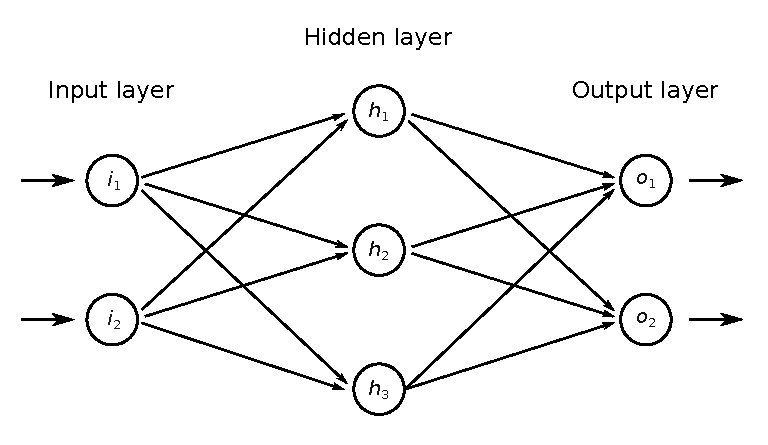
\includegraphics{figures/neuralnetworks.pdf}
    \caption{Schematic drawing of an artificial neural network with three layers}
    \label{fig:neuralnetwork}
\end{figure}
\todo[inline]{Grafik kann nacher noch an unser neuronales Netz angepasst werden}
\cite[4]{BisbySHM} defines SHM to be "a non-destructive \textit{in-situ} structural evaluation method that uses any of several sensors which are attached to, or embedded in, a structure". The obtained data is "collected, analyzed and stored".

%\begin{itemize}
%\item neurons
%\item layer
%\item weights
%\item activation function / identity function
%\end{itemize}

\textbf{2. paragraph: proposed nn}

\begin{itemize}
\item SNIPE? implementation in java?
\item activation function / identity function
\end{itemize}

\textbf{3. paragraph: learning general}

\begin{itemize}
\item set with test values
\item iterative weight adjustment
\end{itemize}

\textbf{4. paragraph?: learning, proposed}

%----------------------------------------------------------------------------------------

\section*{FFT}

\begin{itemize}
\item Frequenzspektrum ermitteln
\end{itemize}


\newpage
\section*{Laboratory experiments}

\textbf{1. paragraph: test setting}

\begin{itemize}
\item test structure, picture
\item sensor installation
\item type of excitation, acceleration is measured

\item learning phase
\end{itemize}

\textbf{2. paragraph: data measurement and processing}

\begin{itemize}
\item excitation
\item sensors start measuring
\item sensor nodes perform fft
\item sensor nodes exchange frequencies
\item neural networks check integrity
\item if no faults detected, sensor nodes send data to base station
\end{itemize}

\textbf{3. paragraph: sensor fault}

\begin{itemize}
\item simulation of sensor fault
\item neural networks check integrity -> error!
\item sensor node sends alert to base station
\end{itemize}

%----------------------------------------------------------------------------------------

\section*{Discussion of the experimental results}

%----------------------------------------------------------------------------------------

\section*{Summary and conclusions}

%----------------------------------------------------------------------------------------
\todo{sie sind da!}

\bibliographystyle{unsrtnat}
\bibliography{literature}

\end{document}




















